\documentclass{article}

\usepackage{courier}
\usepackage{graphicx} % Required for the inclusion of images
\usepackage{listings}
\usepackage{color}
\usepackage{amsmath}
\usepackage{subcaption}
\usepackage{enumitem}
\usepackage{float}
\usepackage[toc,page]{appendix}
\usepackage{dcolumn}
\usepackage{pdflscape}
\usepackage{hyperref}
\usepackage{framed}
\usepackage[english]{babel}
\usepackage{soul}
\usepackage{caption}
\usepackage{amsfonts}
\usepackage{MnSymbol,wasysym}
\usepackage{algorithmic}
\captionsetup[figure]{labelformat=empty}%

\setlength\parindent{0pt} % Removes all indentation from paragraphs

\renewcommand{\labelenumi}{\alph{enumi}.} % Make numbering in the enumerate environment by letter rather than number (e.g. section 6)

\definecolor{dkgreen}{rgb}{0,0.6,0}
\definecolor{gray}{rgb}{0.5,0.5,0.5}
\definecolor{mauve}{rgb}{0.58,0,0.82}

\lstset{frame=tb,
  language=R,
  aboveskip=3mm,
  belowskip=3mm,
  showstringspaces=false,
  columns=flexible,
  basicstyle={\small\ttfamily},
  numbers=none,
  numberstyle=\tiny\color{gray},
  keywordstyle=\color{blue},
  commentstyle=\color{dkgreen},
  stringstyle=\color{mauve},
  breaklines=true,
  breakatwhitespace=true
  tabsize=3
}

\newcommand{\footlabel}[2]{%
    \addtocounter{footnote}{1}%
    \footnotetext[\thefootnote]{%
        \addtocounter{footnote}{-1}%
        \refstepcounter{footnote}\label{#1}%
        #2%
    }%
    $^{\ref{#1}}$%
}

\newcommand{\footref}[1]{%
    $^{\ref{#1}}$%
}

%\usepackage[colorlinks]{hyperref}
\hypersetup{linkcolor=DarkRed}
\hypersetup{urlcolor=DarkBlue}
\usepackage{cleveref}

\title{Data Mining\\Homework Assignment \#11} % Title

\author{Dmytro Fishman, Anna Leontjeva and Jaak Vilo} % Author name

\begin{document}

\maketitle % Insert the title, author and date 
The goal for this homework is to get you started with basics of social network analysis. 

There are many different network analyzing tools. Choose the one you prefer. Some of the well-known tools and packages are: NetworkX and igraph for Python, JUNG for Java, igraph for R, Gephi for the visualization with some built-in calculations and even NodeXL free template for Excel.

Most of the exercises require you to check presentation slides for the definitions.

\section*{Task 1}
In this task, we will use the techniques of Social Network analysis to study a virus spread. Imagine the following situation: terrified biologists came to the Institute of Computer Science seeking for a help. Their email network was infected by the virus that was created by the student that received 'B' for his Master's Thesis and got offended. Your goal is to help poor biologists to estimate the worst-case scenario of this virus spread. 

Biologists observed that if virus infects a node, it always infects all its immediate neighbors, if they are not already infected (100\% of infection rate). Also, we know that virus travels only along the edge direction (e.g. if virus infects node A, which only has an incoming edge from node B, node B will not be infected). 

Biologists provided you with their directed anonymous email network (email\_virus.txt) that you can access on the course web-page. 
  
Load the data. To get the first insights about biologists' network, calculate the list of the following statistics:
\begin{itemize}
\item number of nodes in the network
\item number of edges in the network
\item number of nodes with a self-loop
\item number of mutual connections or \emph{reciprocated} edges, i.e if there is a directed edge from node a to node b, there is also an edge from b to a. 
\item number of nodes with zero indegree (those that have only outgoing edges)
\item number of nodes with zero outdegree (those that have only ingoing edges)
\item degree distribution of the given network
\item optionally calculate whatever measure you deem appropriate for better understanding
\end{itemize}
What intuition you can gather from these numbers?

\section*{Task 2}
Next, biologists ask us to estimate the vulnerability of their network. In order to measure it, you have to calculate average virus spread assuming that the initial infected node is chosen uniformly at random. What is the probability that virus will affect at least 30\% of the network nodes ('large scale' epidemics emerges).

For that, consider the following simplified version of the graph. 
\begin{figure}[H]
    \centering
    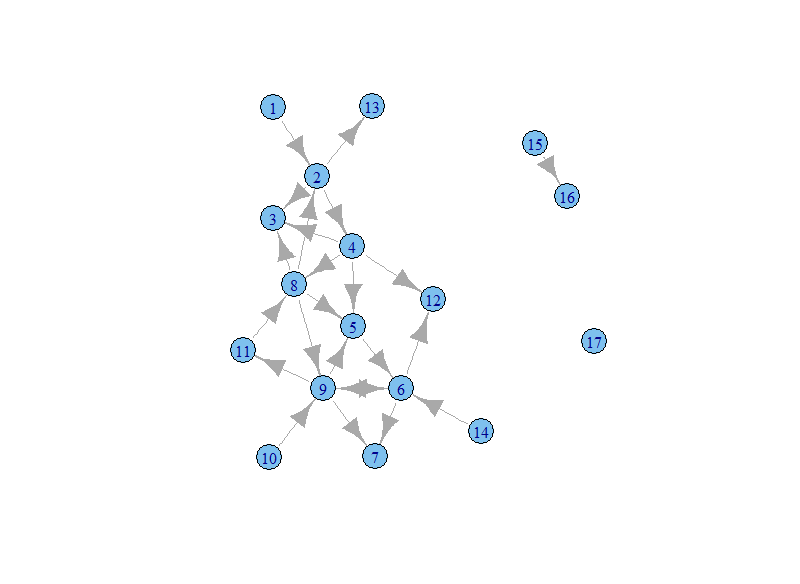
\includegraphics[width=1\textwidth]{Graph.png}
    \caption{Figure: simplified version of the graph}
    \label{fig:awesome_image}
\end{figure}

\begin{enumerate}
\item According to the virus transmission rule, calculate number of infected nodes in three different cases:
\begin{enumerate}
\item  the seed of the infection is node 1
\item the seed of the infection is node 8
\item the seed of the infection is node 12
\end{enumerate} 
\item Here we introduce the notion of Bow Tie structure, which is a recent concept that grasps the essence of both biological networks and the representation of links in the Internet. It divides a graph into 4 basic components (and two secondary that we omit for this task):
\begin{itemize}
\item strongly connected component (SCC), which is the core of the graph, where all nodes can reach one other along directed links
\item  ''IN`` component that consists of nodes that can reach the SCC, but cannot be reached from it.
\item ''OUT`` component that consists of nodes that are accessible from the SCC, but do not link back to it
\item disconnected components are those nodes that are not connected to neither IN, OUT or SCC components. 
\end{itemize}
For more information on described above graph structure read article by Andrei Broder et al.: \url{http://snap.stanford.edu/class/cs224w-readings/broder00bowtie.pdf}\\
In this part, your task is to calculate the proportion of nodes that belong to SCC, IN, OUT and disconnected components.
\item Based on estimated proportions in the part 'b', calculate the probability of emerging a 'large scale' epidemics (at least 30\% of the network nodes infected) given that the initial infected node is chosen uniformly at random from the network nodes.
\end{enumerate}
\section*{Task 3}
In this task we will explore generative mathematical models that try to simulate real-world network according to some characteristics. We will generate three models and compare it with the real-world graph of an academic collaboration network. For that:
\begin{itemize}
\item generate random graph according to Erdos-Renyi model with 5242 nodes and 10484 edges 
\begin{lstlisting}
#Hint for R: use package igraph and function 
erdos.renyi.game(n = 5242, 10484, type = c("gnm"))
#Hint for python library NetworkX: 
gnm_random_graph(5242, 10484)
\end{lstlisting}
\item generate a graph with a small world model (Watts and Strogatz model) so that it has 5242 nodes and 10484 edges. 
\begin{lstlisting}
#In R use function
watts.strogatz.game(1, 5242, 2, 0.5)
#Hint for python NetworkX: 
watts_strogatz_graph(5242, 2, 0.5)
\end{lstlisting}
\item generate preferential attachment model (Barabasi model)
\begin{lstlisting}
#Hint for R: 
barabasi.game(5242, power = 1, m = 2)
#Hint for NetworkX in python 
barabasi_albert_graph(5242, 2)
\end{lstlisting}
\item  load the real collaboration graph undirected\_real\_world\_graph.txt from the course webpage
\end{itemize}
Plot the degree distribution of all three networks both on original and log-log scale. Highly recommended to place all distributions on one plot for comparison. Describe the differences and the shape of the distributions.
 
\section*{Task 4}
The local clustering coefficient for a node $v$ is defined as:
$$C_i = \frac{2|e_i|}{k_i(k_i-1)}$$
where $k_i$ is the degree of $v_i$ and $e_i$ is the number of edges between the neighbors of $v_i$. Your task is to find \emph{average clustering coefficient} that is defined as 
$$C = \frac{1}{|V|}\sum_{i\in V}C_i$$
Note that if a node has 0 or 1 neighbor, we will ignore it.
Calculate average clustering coefficient for all four networks in the previous task. Compare them and describe the difference. 

In case of using built-in functions, one point will be given. If you write a script that calculates average clustering coefficient (instead of built-in function), you will earn additional point.

\section*{Task 5}
In this task you have to come up with your own model for real-world networks generation. Come up with the algorithm and write down the pseudo code for your model. Implement the model and generate the graph of approximately the same size as in previous tasks. Compare degree distribution and clustering coefficient of your graph and other networks.

As an example, you may introduce a notion of nodes dying after some time.
Note that without implementation only half of the point will be given.

\section*{Task 6}
In this bonus task you will help biologists to fight the virus from the task one and two. Use data email\_virus.txt, calculate the same components as in task 2b and the probability of emerging a 'large scale' epidemics as in task 2c. Hint: you may want to use BFS algorithm to estimate IN and OUT components.
\medskip
\\
This homework was inspired by Juri Leskovec stanford course ''Social and Information Network Analysis``. 
\end{document}
